\documentclass[english,11pt,a4paper]{article}
\usepackage[T1]{fontenc} % --------------| More characters.
\usepackage[utf8]{inputenc} % -----------| Direct use of scandinavian letters.
\usepackage{float} % --------------------| More options for floats.
\usepackage{graphicx} % -----------------| Support more image formats.
\usepackage{booktabs} % -----------------| Better-looking tables.
\usepackage{tabularx} % -----------------| Better tables
\usepackage{subcaption} % ---------------| Subfigures.
\usepackage[a4paper]{geometry} % --------| Adjusting page margins.
\usepackage{amsmath,amssymb,amsfonts} % -| Various math, including eqref.
\usepackage{xcolor} % -------------------| Allows defn. of custom colors.
\usepackage{babel}
\usepackage{url}
\usepackage{enumitem}

% XY-pic. Used for creating illustrations.
\input xy
\xyoption{all}

% Styling captions.
\usepackage{caption}
\captionsetup{margin=10pt,font=small,labelfont=bf}


%******************************************************************************
% This preabmle contains packages needed to create figures and plots in LaTeX.
%******************************************************************************

\usepackage{etex}
\usepackage{tikz,pgfplots}
\pgfplotsset{compat=1.9}
\usetikzlibrary{calc}
\usetikzlibrary{fit}
\usetikzlibrary{shapes,snakes}
\usetikzlibrary{arrows,decorations.markings}

% Vector Styles for drawings
\tikzstyle{load}   = [ultra thick,-latex]
\tikzstyle{stress} = [-latex]
\tikzstyle{dim}    = [latex-latex]
\tikzstyle{axis}   = [-latex,black!55]


\tikzset{arrowmid/.style={
        decoration={
            markings,
            mark=at position #1 with {\arrow{>}}},postaction={decorate}
    }
}


\tikzset{three sided bottom/.style={
        draw=none,
        append after command={
            [shorten <= -0.5\pgflinewidth]
            ([shift={(-1.5\pgflinewidth,-0.5\pgflinewidth)}]\tikzlastnode.north east) % North edge
        edge([shift={( 0.5\pgflinewidth,-0.5\pgflinewidth)}]\tikzlastnode.north west) % North edge
            ([shift={(-0.5\pgflinewidth,-0.5\pgflinewidth)}]\tikzlastnode.north east) % East edge
        edge([shift={(-0.5\pgflinewidth,-0.0\pgflinewidth)}]\tikzlastnode.south east) % East edge
            ([shift={( 0.5\pgflinewidth,-0.5\pgflinewidth)}]\tikzlastnode.north west) % West edge
        edge([shift={( 0.5\pgflinewidth,+0.5\pgflinewidth)}]\tikzlastnode.south west) % West edge
            % ([shift={( 0.5\pgflinewidth,+0.5\pgflinewidth)}]\tikzlastnode.south west) % South edge
        % edge([shift={(-1.0\pgflinewidth,+0.5\pgflinewidth)}]\tikzlastnode.south east) % South edge

        }
    }
}

\tikzset{three sided top/.style={
        draw=none,
        append after command={
            [shorten <= -0.5\pgflinewidth]
            % ([shift={(-1.5\pgflinewidth,-0.5\pgflinewidth)}]\tikzlastnode.north east) % North edge
        % edge([shift={( 0.5\pgflinewidth,-0.5\pgflinewidth)}]\tikzlastnode.north west) % North edge
            ([shift={(-0.5\pgflinewidth,-0.5\pgflinewidth)}]\tikzlastnode.north east) % East edge
        edge([shift={(-0.5\pgflinewidth,-0.0\pgflinewidth)}]\tikzlastnode.south east) % East edge
            ([shift={( 0.5\pgflinewidth,-0.5\pgflinewidth)}]\tikzlastnode.north west) % West edge
        edge([shift={( 0.5\pgflinewidth,+0.5\pgflinewidth)}]\tikzlastnode.south west) % West edge
            ([shift={( 0.5\pgflinewidth,+0.5\pgflinewidth)}]\tikzlastnode.south west) % South edge
        edge([shift={(-1.0\pgflinewidth,+0.5\pgflinewidth)}]\tikzlastnode.south east) % South edge

        }
    }
}

\tikzset{rectangle split h/.style={
    draw, rectangle split, rectangle split parts=#1, rectangle split horizontal
}}


\tikzset{underbrace/.style={
    thick,
    decoration={
        brace,
        mirror,
    },
    decorate
}}

\tikzset{overbrace/.style={
    thick,
    decoration={
        brace,
    },
    decorate
}}

\tikzset{overbrace label/.style={
    pos=0.5,anchor=south,yshift=0.2cm
}}

\tikzset{underbrace label/.style={
    pos=0.5,anchor=north,yshift=-0.2cm
}}


\author{Einar Baumann}
\title{
    \vspace{-1in}
    \usefont{OT1}{bch}{b}{n}
    \vspace{0.1in}
    \rule{\textwidth}{0.5pt} \\[0.5cm]
    \normalfont \normalsize \textsc{TPG4160 Reservoir Simulation} \\ [20pt]
    {\textsc{ \huge Exercise 4}} \\
    \vspace{0.1in}
    \rule{\textwidth}{2pt} \\[0.7cm]
}

\begin{document}
\maketitle
\thispagestyle{empty}
\clearpage

\section{Changes to the DATA file} % (fold)
\label{sec:changes_to_the_data_file}
I assumed that ``extending'' the horizonatal grid implied that dx and dy shouldn't be changed. I also assumed that ``refining'' the vertical grid implied that the total thickness of the model should be the same; so I divided the dx-values for each cell by 10.

The most important modified properties in the DATA-file are the following:

\begin{verbatim}
DIMENS
 20   20    30  /

WELLDIMS
    2    10    1    2 /

'DZ'    2         1  20  1  20  1  10 /
'MULTZ' 0.64      1  20  1  20  10  10  /
'DZ'    3         1  20  1  20  11  20  /
'MULTZ' 0.265625  1  20  1  20  20  20  /
'DZ'    5         1  20  1  20  21  30  /

COPY
      'PERMX'    'PERMY'   1  20  1  20  1  30  /

BGSAT
20 20 30
1  1  1
/
BOSAT
20 20 30
1  1  1
/
BPR
20 20 30
1  1  1
/

WELSPECS
    'PRODUCER' 'G'   20 20    8400 'OIL'  /
    'INJECTOR' 'G'    1  1    8335 'GAS'  /
/

COMPDAT
    'PRODUCER'  20 20 21 30 'OPEN' 0   -1   0.5  /
    'INJECTOR'  1  1  1  10  'OPEN' 1   -1   0.5  /
  /
\end{verbatim}
% section changes_to_the_data_file (end)

\section{Interpretation} % (fold)
\label{sec:interpretation}
The gas-oil ratio is shown in Figure~\ref{fig:gor} and the oil production rate is shown in Figure~\ref{fig:opr}. In both plots we see that the lines do not move away from the steady plateau-production for the new, larger grid. This is likely due to the new reservoir having a larger volume, which means that the reservoir won't reach bubble-point pressure until a later date.

The plots are made by copying the data from s3graf in table form, modifying the formatting slightly, and using it as input to tikz/pgfplots.

The grid with pressure is shown in Figure~\ref{fig:grid} for reference.
% section interpretation (end)



\begin{figure}[htbp]
  \centering
  \includegraphics{illustrations/gor.pdf}
  \caption{Plot of gas-oil ratio for two different grids.}
  \label{fig:gor}
\end{figure}

\begin{figure}[htbp]
  \centering
  \includegraphics{illustrations/opr.pdf}
  \caption{Plot of oil production rate for two different grids.}
  \label{fig:opr}
\end{figure}

\begin{figure}[htbp]
  \centering
  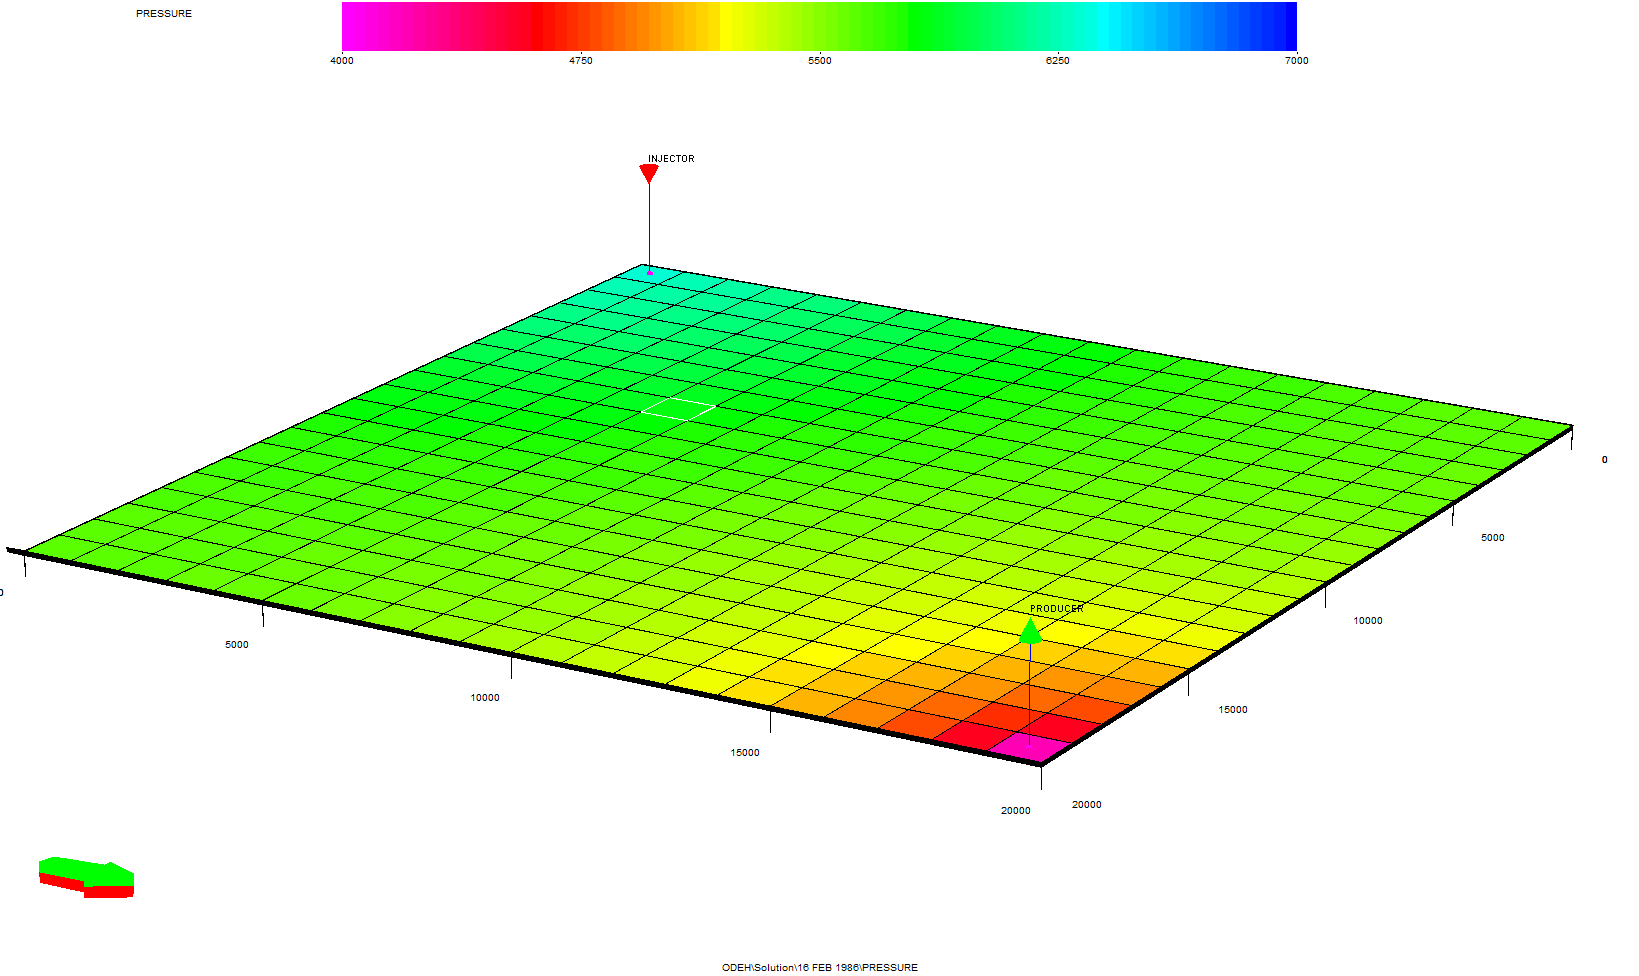
\includegraphics[width=0.95\textwidth]{illustrations/grid.png}
  \caption{The grid with pressure at the initial date shown.}
  \label{fig:grid}
\end{figure}

\end{document}
